


\chapter{Teoretyczne podstawy estymacji FTP i przegląd literatury (rozdział teoretyczno-literaturowy)}

Wydolność tlenowa w kolarstwie jest jednym z kluczowych czynników determinujących wynik sportowy \parencite{borszcz2018ftp}.
Jej ilościowy opis od lat stanowi przedmiot badań fizjologów wysiłku i trenerów.
W praktyce treningowej potrzebne są wskaźniki, które z jednej strony dobrze odzwierciedlają możliwości zawodnika, a z drugiej są możliwe do regularnego monitorowania w warunkach terenowych.
Jednym z najczęściej stosowanych parametrów jest funkcjonalny próg mocy (ang.\ \textit{Functional Threshold Power}, $\mathrm{FTP}$) \parencite{borszcz2018ftp,allen2019power,gavin2012ftp_lt_field}.

Rozwój czujników pomiaru mocy, opasek rejestrujących tętno oraz szerokie wykorzystanie liczników rowerowych i platform treningowych powoduje, że powstają liczne zbiory danych treningowych.
Dane te mogą zostać wykorzystane w modelach uczenia maszynowego do estymacji $\mathrm{FTP}$ na podstawie codziennych jazd, bez potrzeby wykonywania osobnych, wyczerpujących testów.

W niniejszym rozdziale przedstawiono podstawowe pojęcia związane z $\mathrm{FTP}$, charakterystykę danych wykorzystywanych w dalszej części pracy, klasyczne i oparte na uczeniu maszynowym metody szacowania parametrów wydolnościowych oraz przegląd badań i istniejących rozwiązań.

\section{FTP jako parametr wydolności}

Funkcjonalny próg mocy ($\mathrm{FTP}$) jest jednym z najczęściej stosowanych w praktyce treningowej wskaźników wydolności tlenowej kolarzy \parencite{borszcz2018ftp,allen2019power}.
Intuicyjnie można go opisać jako „moc, którą kolarz jest w stanie utrzymać przez dłuższy czas bez narastającego, gwałtownego zmęczenia”.
W przeciwieństwie do prostych wartości maksymalnych (np.\ maksymalnej mocy szczytowej czy tętna maksymalnego), $\mathrm{FTP}$ odnosi się do zdolności organizmu do długotrwałego utrzymania wysokiej, ale jeszcze zrównoważonej intensywności wysiłku.
Z tego powodu parametr ten dobrze nadaje się do opisu poziomu sportowego i planowania treningu wytrzymałościowego.

\subsection{Definicja funkcjonalnego progu mocy}

W literaturze związanej z treningiem kolarskim parametr $\mathrm{FTP}$ najczęściej definiuje się jako najwyższą wartość mocy, jaką kolarz jest w stanie utrzymać w stanie quasi-stacjonarnym przez około $60$ minut \parencite{borszcz2018ftp,allen2019power}.
„Quasi-stacjonarny” oznacza tutaj, że reakcja fizjologiczna organizmu (w szczególności tętno, wentylacja oraz stężenie mleczanu we krwi) stabilizują się na podwyższonym, ale względnie stałym poziomie.
W praktyce przyjmuje się, że przy mocy równej $\mathrm{FTP}$ parametry te nie narastają już gwałtownie, natomiast przekroczenie tej intensywności prowadzi do szybkiego narastania zmęczenia i konieczności zredukowania mocy \parencite{borszcz2018ftp,karsten2021cpftp}.

Ze względów praktycznych $\mathrm{FTP}$ rzadko wyznacza się z pełnego, $60$-minutowego testu czasowego.
Taki test jest bardzo obciążający, wymaga odpowiednich warunków i trudno go często powtarzać.
Dlatego w treningu amatorskim i zawodowym spopularyzowały się krótsze protokoły, z których najpopularniejszy jest $20$-minutowy test maksymalny \parencite{allen2019power}.
Uproszczona wersja polega na wykonaniu rozgrzewki, a następnie jeździe z maksymalnym możliwym wysiłkiem  przez $20$ minut.
Średnia moc z tego odcinka jest następnie mnożona przez współczynnik (najczęściej $0{,}95$), co ma przybliżać moc, jaką kolarz byłby w stanie utrzymać przez $60$ minut \parencite{allen2019power,sitko2023_ac20to60_update,inglis2020ftp_mlss}.

\begin{equation}
\label{eq:ftp_20min}
\mathrm{FTP} \approx 0{,}95 \cdot \overline{P}_{20\ \mathrm{min}},
\end{equation}
gdzie $\overline{P}_{20\ \mathrm{min}}$ oznacza średnią moc w $20$-minutowym odcinku testowym.

Współczynnik $0{,}95$ należy traktować jako praktyczną heurystykę, a nie jako uniwersalne prawo fizjologiczne. Różnica pomiędzy maksymalną mocą możliwą do utrzymania przez $20$ i $60$ minut zależy między innymi od profilu zawodnika, poziomu wytrenowania, zdolności do wysiłków o dużej intensywności oraz umiejętności rozłożenia tempa. Kolarz o relatywnie silnym komponencie beztlenowym może osiągnąć bardzo dobry wynik krótszej próby, który po prostym przemnożeniu będzie zawyżał wartość odpowiadającą wysiłkowi godzinnemu. U innej osoby relacja może być bliższa przyjętemu przelicznikowi. Zmienność tę opisują badania porównujące próby 20- i 60-minutowe \parencite{sitko2023_ac20to60_update,gough2025reliability}.

Warto podkreślić, że jest to definicja funkcjonalna, a nie „fizjologiczna” w ścisłym sensie.
$\mathrm{FTP}$ nie jest bezpośrednim pomiarem żadnego pojedynczego mechanizmu w organizmie (np.\ maksymalnego poboru tlenu), lecz wygodnym parametrem łączącym w sobie kilka aspektów wydolności: zdolność do generowania mocy, tolerancję zmęczenia i efektywność procesów metabolicznych \parencite{borszcz2018ftp,karsten2021cpftp}.

W tym miejscu konieczne jest rozróżnienie kilku pojęć stosowanych w diagnostyce wysiłkowej. Moc krytyczna ($\mathrm{CP}$) jest parametrem modelu matematycznego opisującego relację pomiędzy możliwą do utrzymania mocą a czasem wysiłku. Maksymalny stan równowagi mleczanowej (ang.\ \textit{Maximal Lactate Steady State}, $\mathrm{MLSS}$) odnosi się natomiast do najwyższej intensywności, przy której stężenie mleczanu może pozostawać względnie stabilne podczas wysiłku ciągłego. Progi mleczanowe ($\mathrm{LT}_1$, $\mathrm{LT}_2$) i wentylacyjne ($\mathrm{VT}_1$, $\mathrm{VT}_2$) są wyznaczane na podstawie zmian odpowiednio stężenia mleczanu lub parametrów oddechowych podczas próby o narastającym obciążeniu. Wszystkie te wskaźniki opisują obszar przemian energetycznych istotny dla wysiłku wytrzymałościowego, lecz nie są synonimami FTP \parencite{jones2019mmss,borszcz2018ftp,karsten2021cpftp,mcgrath2021cpftp,jeffries2021ftp_lt,caen2024cp_mlss,chorley2020cpReview,galanRioja2020cpThresholds}.

Różnica ma znaczenie praktyczne. Zawodnik może uzyskać podobne wartości kilku wskaźników, ale ich zgodność nie jest zagwarantowana na poziomie indywidualnym. FTP ma przede wszystkim wartość funkcjonalną: umożliwia planowanie treningu na podstawie mocy rejestrowanej na rowerze. CP wynika z dopasowania modelu do kilku wysiłków, a progi fizjologiczne wymagają obserwacji reakcji organizmu w określonym protokole. Posługiwanie się tymi terminami zamiennie prowadziłoby do nadmiernego uproszczenia i mogłoby sugerować precyzję, której pojedynczy pomiar nie zapewnia.

Heurystyczny charakter przelicznika jest istotny również dla dalszej części pracy. Jeżeli etykieta modelu zostaje utworzona z maksymalnej średniej mocy 20-minutowej, model uczy się przybliżać właśnie tak zdefiniowaną wartość referencyjną. Nie oznacza to automatycznie, że estymuje bezpośrednio $\mathrm{MLSS}$, $\mathrm{CP}$ albo wynik pełnego testu godzinnego. Rozróżnienie pomiędzy etykietą operacyjną a konstruktem fizjologicznym pozwala ostrożnie interpretować jakość predykcji.

\subsection{Pomiar mocy w kolarstwie}

Upowszechnienie mierników mocy stanowi jeden z kluczowych czynników umożliwiających rozwój ilościowej analizy treningu kolarskiego. W przeciwieństwie do prędkości, która jest silnie zależna od warunków zewnętrznych (takich jak siła i kierunek wiatru, nachylenie terenu czy opory toczenia), moc stanowi bezpośrednią i obiektywną miarę pracy mechanicznej wykonywanej przez zawodnika.

Pomiar mocy w kolarstwie opiera się zazwyczaj na rejestracji siły lub momentu obrotowego w wybranym elemencie układu napędowego roweru. Najpopularniejsze rozwiązania techniczne umiejscawiają czujniki w pedałach, ramionach korby, pająku korby, osi suportu lub w piaście tylnego koła \parencite{luder2024cyclowatt}. Zasadniczym elementem pomiarowym w tego typu urządzeniach są tensometry. Te rezystancyjne czujniki rejestrują mikroskopijne odkształcenia elementów konstrukcyjnych pod wpływem nacisku stóp kolarza, co pozwala wyznaczyć siłę reakcji i moment obrotowy \parencite{bouillod2022powerMeters}. Poprzez połączenie tych wartości z kadencją (częstością obrotów korby) wyznacza się chwilową moc mechaniczną wyrażoną w watach.

Warto podkreślić, że miejsce instalacji czujnika wpływa na charakterystykę uzyskiwanych pomiarów. Mierniki zlokalizowane w pedałach lub ramionach korby mierzą moc bardzo blisko punktu przyłożenia siły, co minimalizuje wpływ strat mechanicznych w układzie napędowym (np.\ strat na łańcuchu czy łożyskach). Pozwala to również na niezależny pomiar mocy dla lewej i prawej nogi (tzw.\ pomiar obustronny), co umożliwia analizę asymetrii i techniki pedałowania. Z kolei mierniki umieszczone w piaście rejestrują użyteczną moc napędową przekazywaną bezpośrednio na koło, jednak ich wskazania są z natury pomniejszone o straty napędu.

Rozwój technologii produkcji, miniaturyzacja układów scalonych oraz popularyzacja energooszczędnych protokołów transmisji bezprzewodowej (takich jak ANT+ czy Bluetooth Low Energy) spowodowały, że urządzenia te stały się znacznie tańsze, bardziej niezawodne i szerzej dostępne dla amatorów. Wczesne systemy pomiarowe były zarezerwowane głównie dla profesjonalistów i laboratóriów badawczych z uwagi na zaporowe ceny i skomplikowaną obsługę. Współczesne mierniki cechują się dokładnością deklarowaną przez producentów w granicach $1-2\%$ oraz posiadają wbudowane algorytmy aktywnej kompensacji wpływu temperatury w celu zapobiegania tzw.\ dryfowi zera \parencite{bouillod2022powerMeters}.

Z punktu widzenia analizy danych i uczenia maszynowego kluczowy jest fakt, że mierniki mocy standardowo próbkują i przesyłają dane z częstotliwością $1\ \mathrm{Hz}$. Rejestrowany ciąg wartości tworzy gęsty szereg czasowy, który szczegółowo odwzorowuje strukturę wysiłku kolarza. Sygnał mocy charakteryzuje się jednak dużą zmiennością, występowaniem tzw.\ szumu, krótkotrwałymi pikami mocy oraz licznymi wartościami zerowymi wynikającymi z jazdy bez pedałowania (np.\ na zjazdach lub przed zakrętami). Ocena wiarygodności urządzenia powinna uwzględniać dokładność, czułość, powtarzalność, odtwarzalność i odporność na warunki pomiaru \parencite{bouillod2022powerMeters}. Dodatkowym źródłem błędu systematycznego mogą być mierniki jednostronne, które estymują moc całkowitą na podstawie pomiaru jednej kończyny i założenia symetrii pedałowania \parencite{valenzuela2022unilateral}. Popularyzacja mierników wygenerowała ogromną ilość rzeczywistych danych treningowych, które mogą być gromadzone w platformach sportowych i wykorzystywane w badaniach przekrojowych. Dostępność tych bogatych zbiorów ma bezpośrednie znaczenie dla badań wykorzystujących metody uczenia maszynowego do estymacji parametrów wydolnościowych, zapewniając odpowiednią wielkość próby do trenowania złożonych modeli predykcyjnych.

\subsection{Znaczenie pomiaru mocy w treningu kolarskim}

Współczesny trening kolarski coraz częściej opiera się na pomiarze mocy generowanej przez zawodnika.
W przeciwieństwie do tętna czy subiektywnego odczucia wysiłku ($\mathrm{RPE}$), moc jest parametrem bezpośrednio opisującym pracę mechaniczną wykonywaną na rowerze.
Informuje wprost, ile energii w jednostce czasu kolarz przekazuje na napędzanie roweru, niezależnie od takich czynników jak stres, temperatura otoczenia czy chwilowe wahania nastroju \parencite{allen2019power,phasescycling2023_ftp_variability}.

Pomiar mocy ma kilka kluczowych zalet z punktu widzenia planowania i analizy treningu:
\begin{itemize}
  \item \textbf{Obiektywność i powtarzalność} - ta sama wartość mocy oznacza ten sam poziom obciążenia zewnętrznego, niezależnie od dnia i samopoczucia zawodnika. Ułatwia to porównywanie wysiłków w czasie oraz między różnymi jednostkami treningowymi.
  \item \textbf{Dokładne sterowanie intensywnością} - strefy treningowe oparte na procentach $\mathrm{FTP}$ pozwalają precyzyjnie dozować obciążenie (np.\ trening progowy, $\text{VO}_{2\max}$, jazdy regeneracyjne), co sprzyja świadomemu kształtowaniu określonych adaptacji fizjologicznych \parencite{allen2019power}.
  \item \textbf{Lepsza analiza obciążeń niż na podstawie tętna} - tętno reaguje z opóźnieniem i podlega wpływowi temperatury, odwodnienia czy stresu. Moc zmienia się natychmiast po zmianie nacisku na pedały, dzięki czemu lepiej odzwierciedla przebieg wysiłku.
  \item \textbf{Możliwość zaawansowanej analizy danych} - rejestracja mocy w czasie pozwala obliczać wskaźniki (np.\ moc znormalizowana $\mathrm{NP}$, $\mathrm{TSS}$, czas spędzony w strefach), a także stosować modele matematyczne i metody uczenia maszynowego \parencite{stockwell2023mlftp,denham2020predictftp}.
  \item \textbf{Monitorowanie postępu i zmęczenia} - analiza danych z codziennych treningów umożliwia szacowanie zmian $\mathrm{FTP}$ i ogólnego poziomu wytrenowania bez konieczności częstego wykonywania formalnych testów laboratoryjnych \parencite{borszcz2018ftp,karsten2021cpftp,denham2020predictftp}.
\end{itemize}

Z tych powodów moc stała się jednym z podstawowych parametrów używanych w treningu kolarskim na każdym poziomie zaawansowania - od amatorów po zawodowców.
W kontekście niniejszej pracy jest to szczególnie istotne, ponieważ $\mathrm{FTP}$ pełni rolę kluczowego wskaźnika wydolności opartego właśnie na danych z pomiaru mocy.

\subsection{Znaczenie FTP w praktyce treningowej}

$\mathrm{FTP}$ jest szeroko stosowane zarówno w badaniach naukowych, jak i w codziennej praktyce trenerów i kolarzy \parencite{borszcz2018ftp,allen2019power,karsten2021cpftp,denham2020predictftp}.
Wartość tego parametru służy przede wszystkim do:
\begin{itemize}
  \item wyznaczania stref treningowych - zakresy mocy (lub tętna) definiuje się jako procent $\mathrm{FTP}$, co pozwala opisywać intensywność treningu w sposób bardziej obiektywny niż wyłącznie na podstawie odczuć;
  \item monitorowania postępów - wzrost $\mathrm{FTP}$ (np.\ z $250\ \mathrm{W}$ do $270\ \mathrm{W}$) w pewnym okresie czasu interpretuje się jako poprawę wydolności tlenowej;
  \item porównywania zawodników - przeliczenie $\mathrm{FTP}$ na wartość względną $\mathrm{W\,kg^{-1}}$ pozwala porównywać kolarzy o różnej masie ciała;
  \item planowania strategii wyścigowych - znajomość $\mathrm{FTP}$ pomaga oszacować tempo możliwe do utrzymania na długich podjazdach czy w jeździe indywidualnej na czas.
\end{itemize}

Z punktu widzenia uczenia maszynowego $\mathrm{FTP}$ jest naturalnym kandydatem na zmienną wyjściową (etykietę, $y$) w modelach regresyjnych.
Oznacza to, że model ma za zadanie przybliżyć zależność pomiędzy zarejestrowanymi danymi z treningów (moc, tętno, czas, parametry trasy) a „ukrytą” wartością $\mathrm{FTP}$ danego zawodnika \parencite{stockwell2023mlftp,denham2020predictftp}.

\subsection{Podstawy fizjologii wysiłku istotne dla interpretacji FTP}

Aby poprawnie interpretować dane używane przez model oraz ograniczenia tradycyjnych testów $\mathrm{FTP}$, wystarczy uproszczony obraz fizjologii wysiłku:
\begin{itemize}
  \item \textbf{Układ krążenia i tlen.} W trakcie wysiłku mięśnie potrzebują tlenu do wytwarzania energii. Serce pompuje krew bogatą w tlen, a tętno rośnie wraz z intensywnością wysiłku. W średnich intensywnościach wzrost mocy często wiąże się z niemal liniowym wzrostem tętna.
  \item \textbf{Progi metaboliczne.} Przy coraz większej intensywności organizm w coraz większym stopniu korzysta z procesów beztlenowych, a we krwi kumuluje się mleczan. W okolicach progów mleczanowych lub wentylacyjnych równowaga pomiędzy produkcją a usuwaniem mleczanu jest na granicy: organizm jest jeszcze w stanie utrzymać wysiłek, ale przy dalszym zwiększaniu obciążenia równowaga się załamuje i dochodzi do szybkiego narastania zmęczenia. $\mathrm{FTP}$ jest zwykle zlokalizowane w pobliżu tych progów, ale nie jest z nimi tożsame \parencite{borszcz2018ftp,karsten2021cpftp,denham2020predictftp}.
  \item \textbf{Dryf tętna.} Podczas dłuższych wysiłków przy stałej mocy często obserwuje się zjawisko stopniowego wzrostu tętna w czasie, mimo że moc nie rośnie. Wynika to m.in.\ z narastającego zmęczenia, zmian w termoregulacji i niewielkiego spadku objętości krwi krążącej. Oznacza to, że relacja „moc--tętno” nie jest idealnie stała: ta sama moc po $5$ minutach i po $40$ minutach może odpowiadać innemu tętnu. Ponadto tętno reaguje na zmiany mocy z pewnym opóźnieniem, więc po nagłym zwiększeniu lub zmniejszeniu obciążenia serce potrzebuje zwykle kilkudziesięciu sekund, aby „dogonić” nowy poziom wysiłku. Z punktu widzenia modeli uczonych na danych sekunda-po-sekundzie oznacza to, że bieżąca wartość tętna odzwierciedla raczej średnie obciążenie z ostatnich kilkudziesięciu sekund niż chwilowy odczyt mocy.
  \item \textbf{Zmęczenie i wyczerpanie.} Gdy intensywność przekracza zdolność organizmu do stabilnego utrzymania równowagi metabolicznej, narastające zmęczenie prowadzi do konieczności zmniejszenia mocy. W testach $\mathrm{FTP}$ objawia się to przerwaniem wysiłku lub znaczącym obniżeniem mocy, co widać jako spadek mocy na wykresie \parencite{borszcz2018ftp,karsten2021cpftp}.
\end{itemize}

Zjawisko dryfu tętna przy stałej mocy oraz opóźnienie reakcji tętna po zmianie intensywności przedstawiono na rysunku~\ref{fig:hr_drift_hr_lag}.

\begin{figure}[htbp]
  \centering
  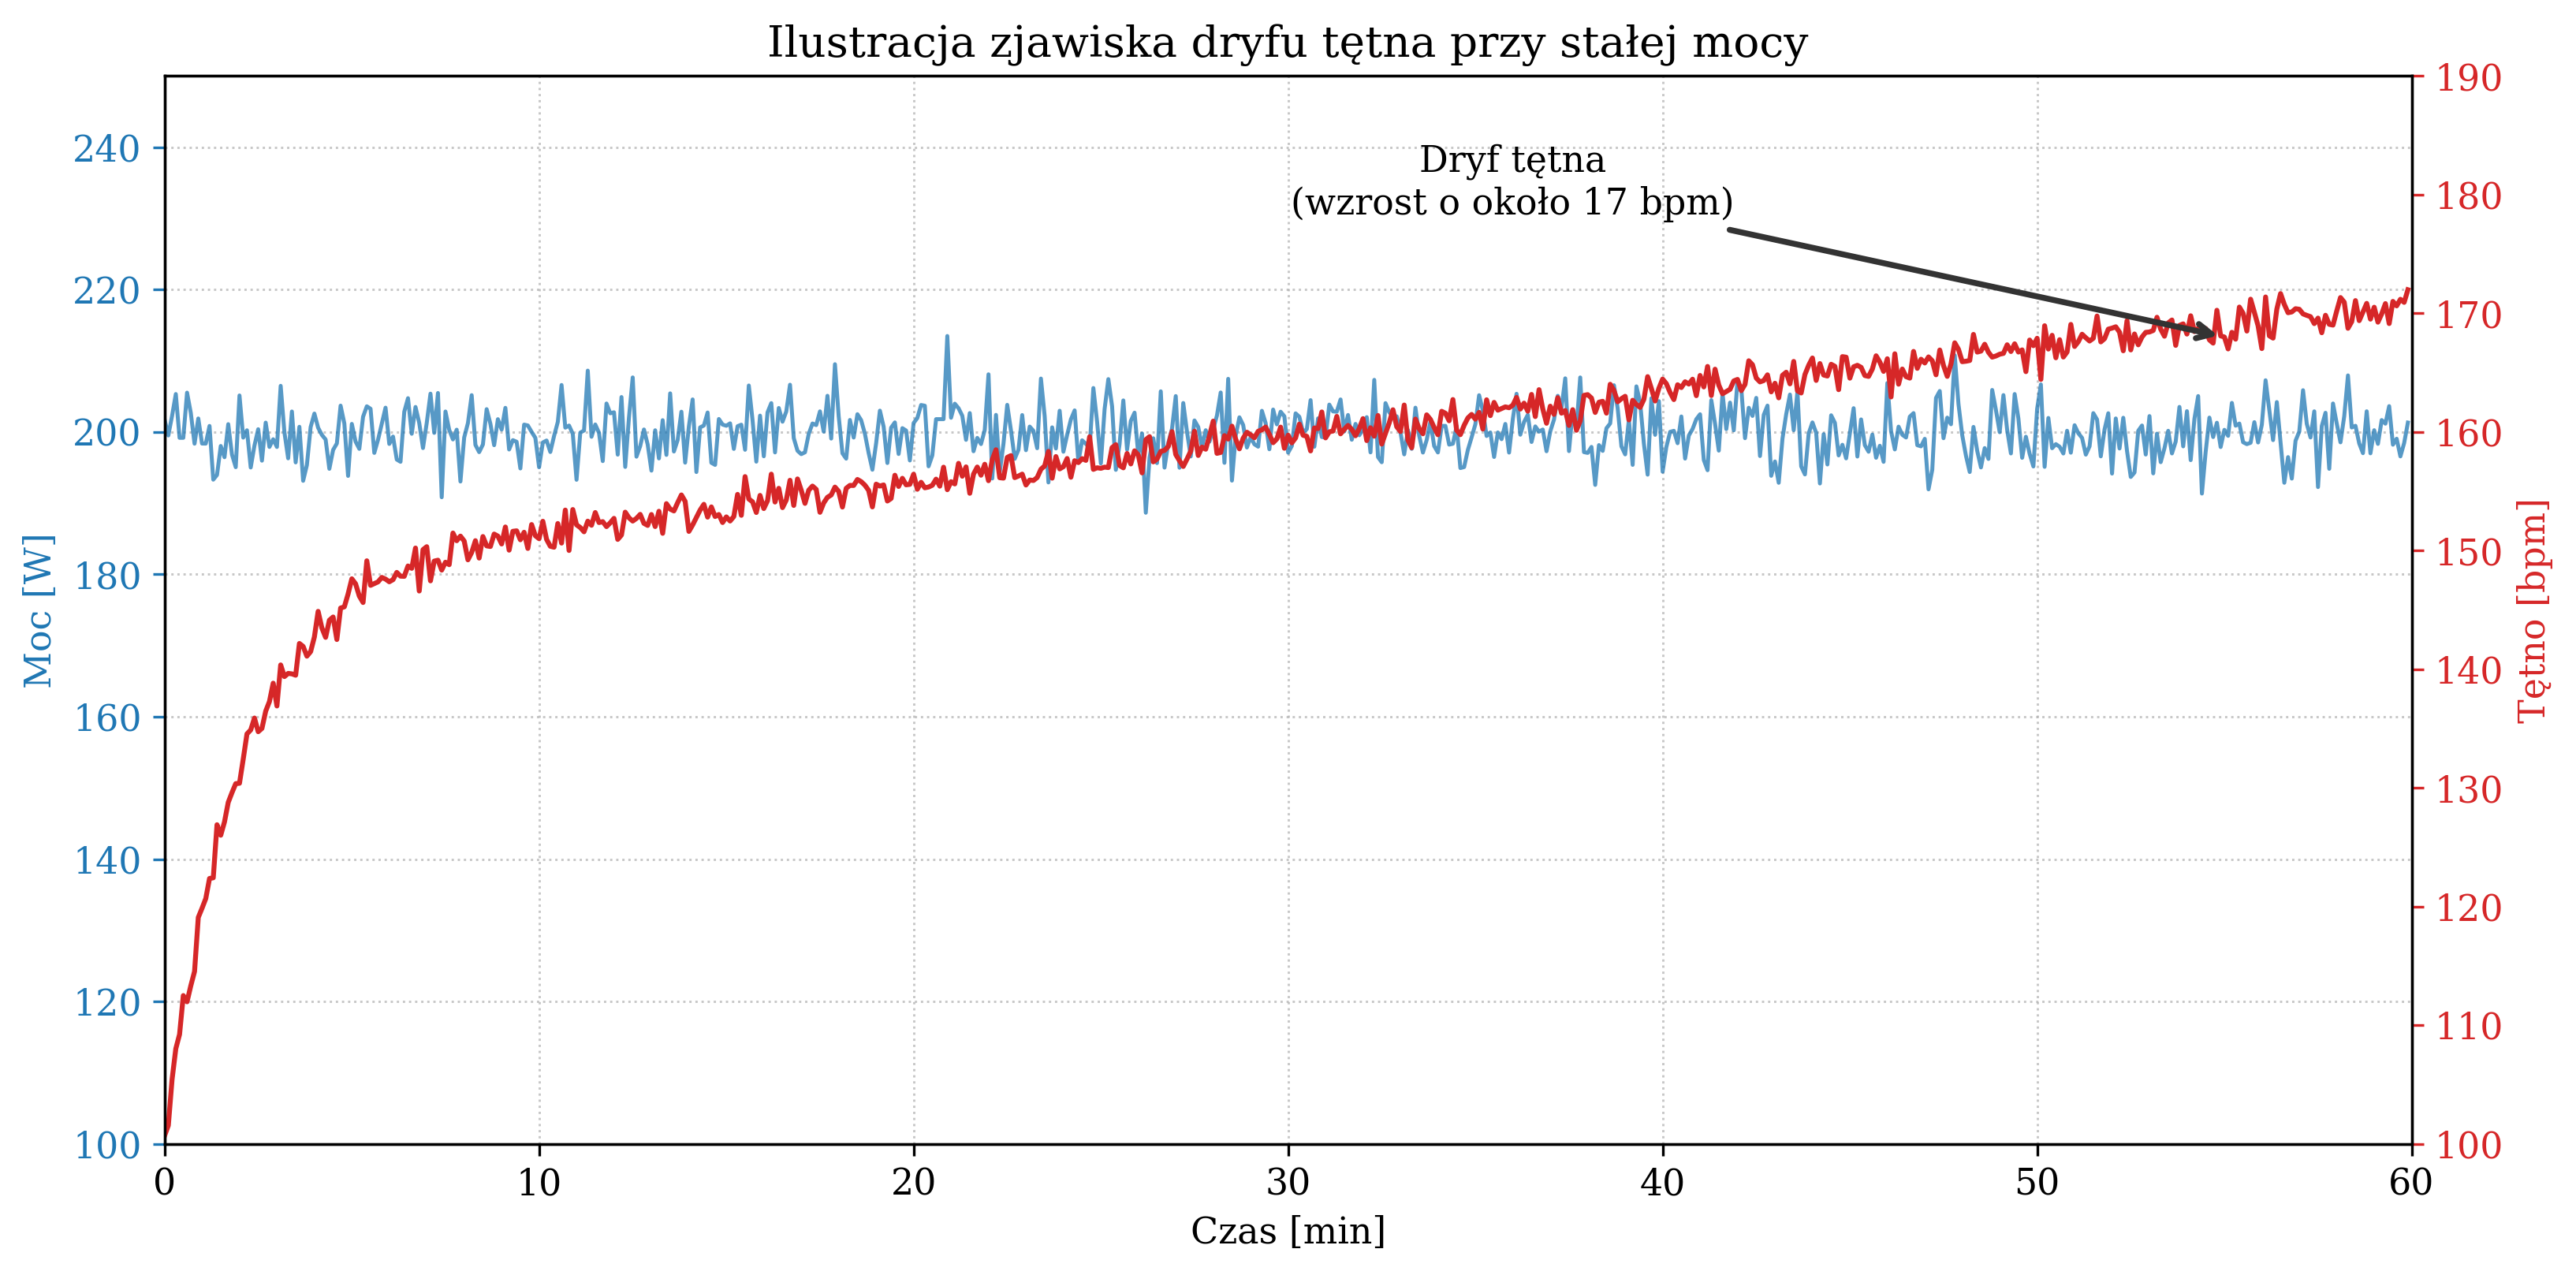
\includegraphics[width=0.95\linewidth]{figures/theory/cardiac_drift.png}
  \caption[Ilustracja zjawiska dryfu tętna przy stałej mocy]{Ilustracja zjawiska dryfu tętna przy stałej mocy oraz widoczne opóźnienie narastania tętna w początkowej fazie wysiłku.\par Źródło: Opracowanie własne na podstawie \parencite{nomadfrontiers_power_hr,bikeradar_power_hr}.}
  \label{fig:hr_drift_hr_lag}
\end{figure}
\FloatBarrier

Z perspektywy modelu uczenia maszynowego oznacza to, że:
\begin{itemize}
  \item sygnał tętna zawiera informację o reakcji organizmu na obciążenie (moc),
  \item relacja moc--tętno jest nieliniowa i zmienia się w czasie (dryf, narastające zmęczenie),
  \item pojedynczy test $\mathrm{FTP}$ jest jedynie pojedynczym pomiarem tej relacji w konkretnych warunkach oraz w konkretnym dniu.
\end{itemize}

Dlatego sensowne jest podejście, w którym model uczy się tej relacji z wielu treningów, zamiast polegać wyłącznie na jednym teście \parencite{stockwell2023mlftp,denham2020predictftp}.

Interpretacja wskaźników fizjologicznych wymaga także rozróżnienia ich funkcji. Pułap tlenowy $\text{VO}_{2\max}$ opisuje maksymalną zdolność organizmu do poboru i wykorzystania tlenu, ale sam nie określa mocy możliwej do długotrwałego utrzymania. Progi $\text{VT}_1$ i $\text{VT}_2$ identyfikuje się na podstawie zmian wentylacji oraz wymiany gazowej, natomiast $\text{LT}_1$ i $\text{LT}_2$ na podstawie przebiegu stężenia mleczanu. FTP jest związane z tym samym ogólnym obszarem wydolności, lecz stanowi wskaźnik terenowy i treningowy. Z tego powodu estymacja FTP z telemetrii jest użyteczna praktycznie, ale nie zastępuje pełnej diagnostyki laboratoryjnej.

\subsection{Test 20-minutowy -- przebieg i ilustracja}

Najpopularniejszy protokół używany w praktyce do wyznaczania $\mathrm{FTP}$ to test $20$-minutowy \parencite{allen2019power,sitko2023_ac20to60_update,phasescycling2023_ftp_variability}.
W praktyce treningowej standardowy protokół testowy, zaproponowany m.in. przez Allena i Coggana \parencite{allen2019power}, składa się z kilku następujących po sobie faz o ściśle określonym celu fizjologicznym:
\begin{itemize}
  \item \textbf{Faza wprowadzenia (rozgrzewka)} -- obejmuje 10--20 minut jazdy o niskiej i umiarkowanej intensywności w celu pobudzenia układu krążeniowo-oddechowego.
  \item \textbf{Faza adaptacji (wysiłek przygotowawczy)} -- polega na wykonaniu krótkiego (zwykle 3--5 minut) wysiłku o intensywności przewyższającej próg w celu wyczerpania komponentu beztlenowego przed próbą główną.
  \item \textbf{Faza regeneracji bezpośredniej} -- kilkunastominutowy etap spokojnej jazdy ułatwiający utylizację mleczanu przed rozpoczęciem testu.
  \item \textbf{Próba zasadnicza} -- 20-minutowy wysiłek maksymalny o stałej intensywności, podczas którego rejestrowana jest średnia moc stanowiąca bazę do wyznaczenia FTP.
\end{itemize}

Schemat przebiegu testu $20$-minutowego zaprezentowano na rysunku~\ref{fig:test_20min_schema}.
Schemat obejmuje rozgrzewkę, krótki wysiłek pobudzający, fragment spokojnej jazdy, właściwy test w postaci dwudziestu minut możliwie równego wysiłku oraz odpoczynek w formie rozjazdu.

\begin{figure}[htbp]
  \centering
  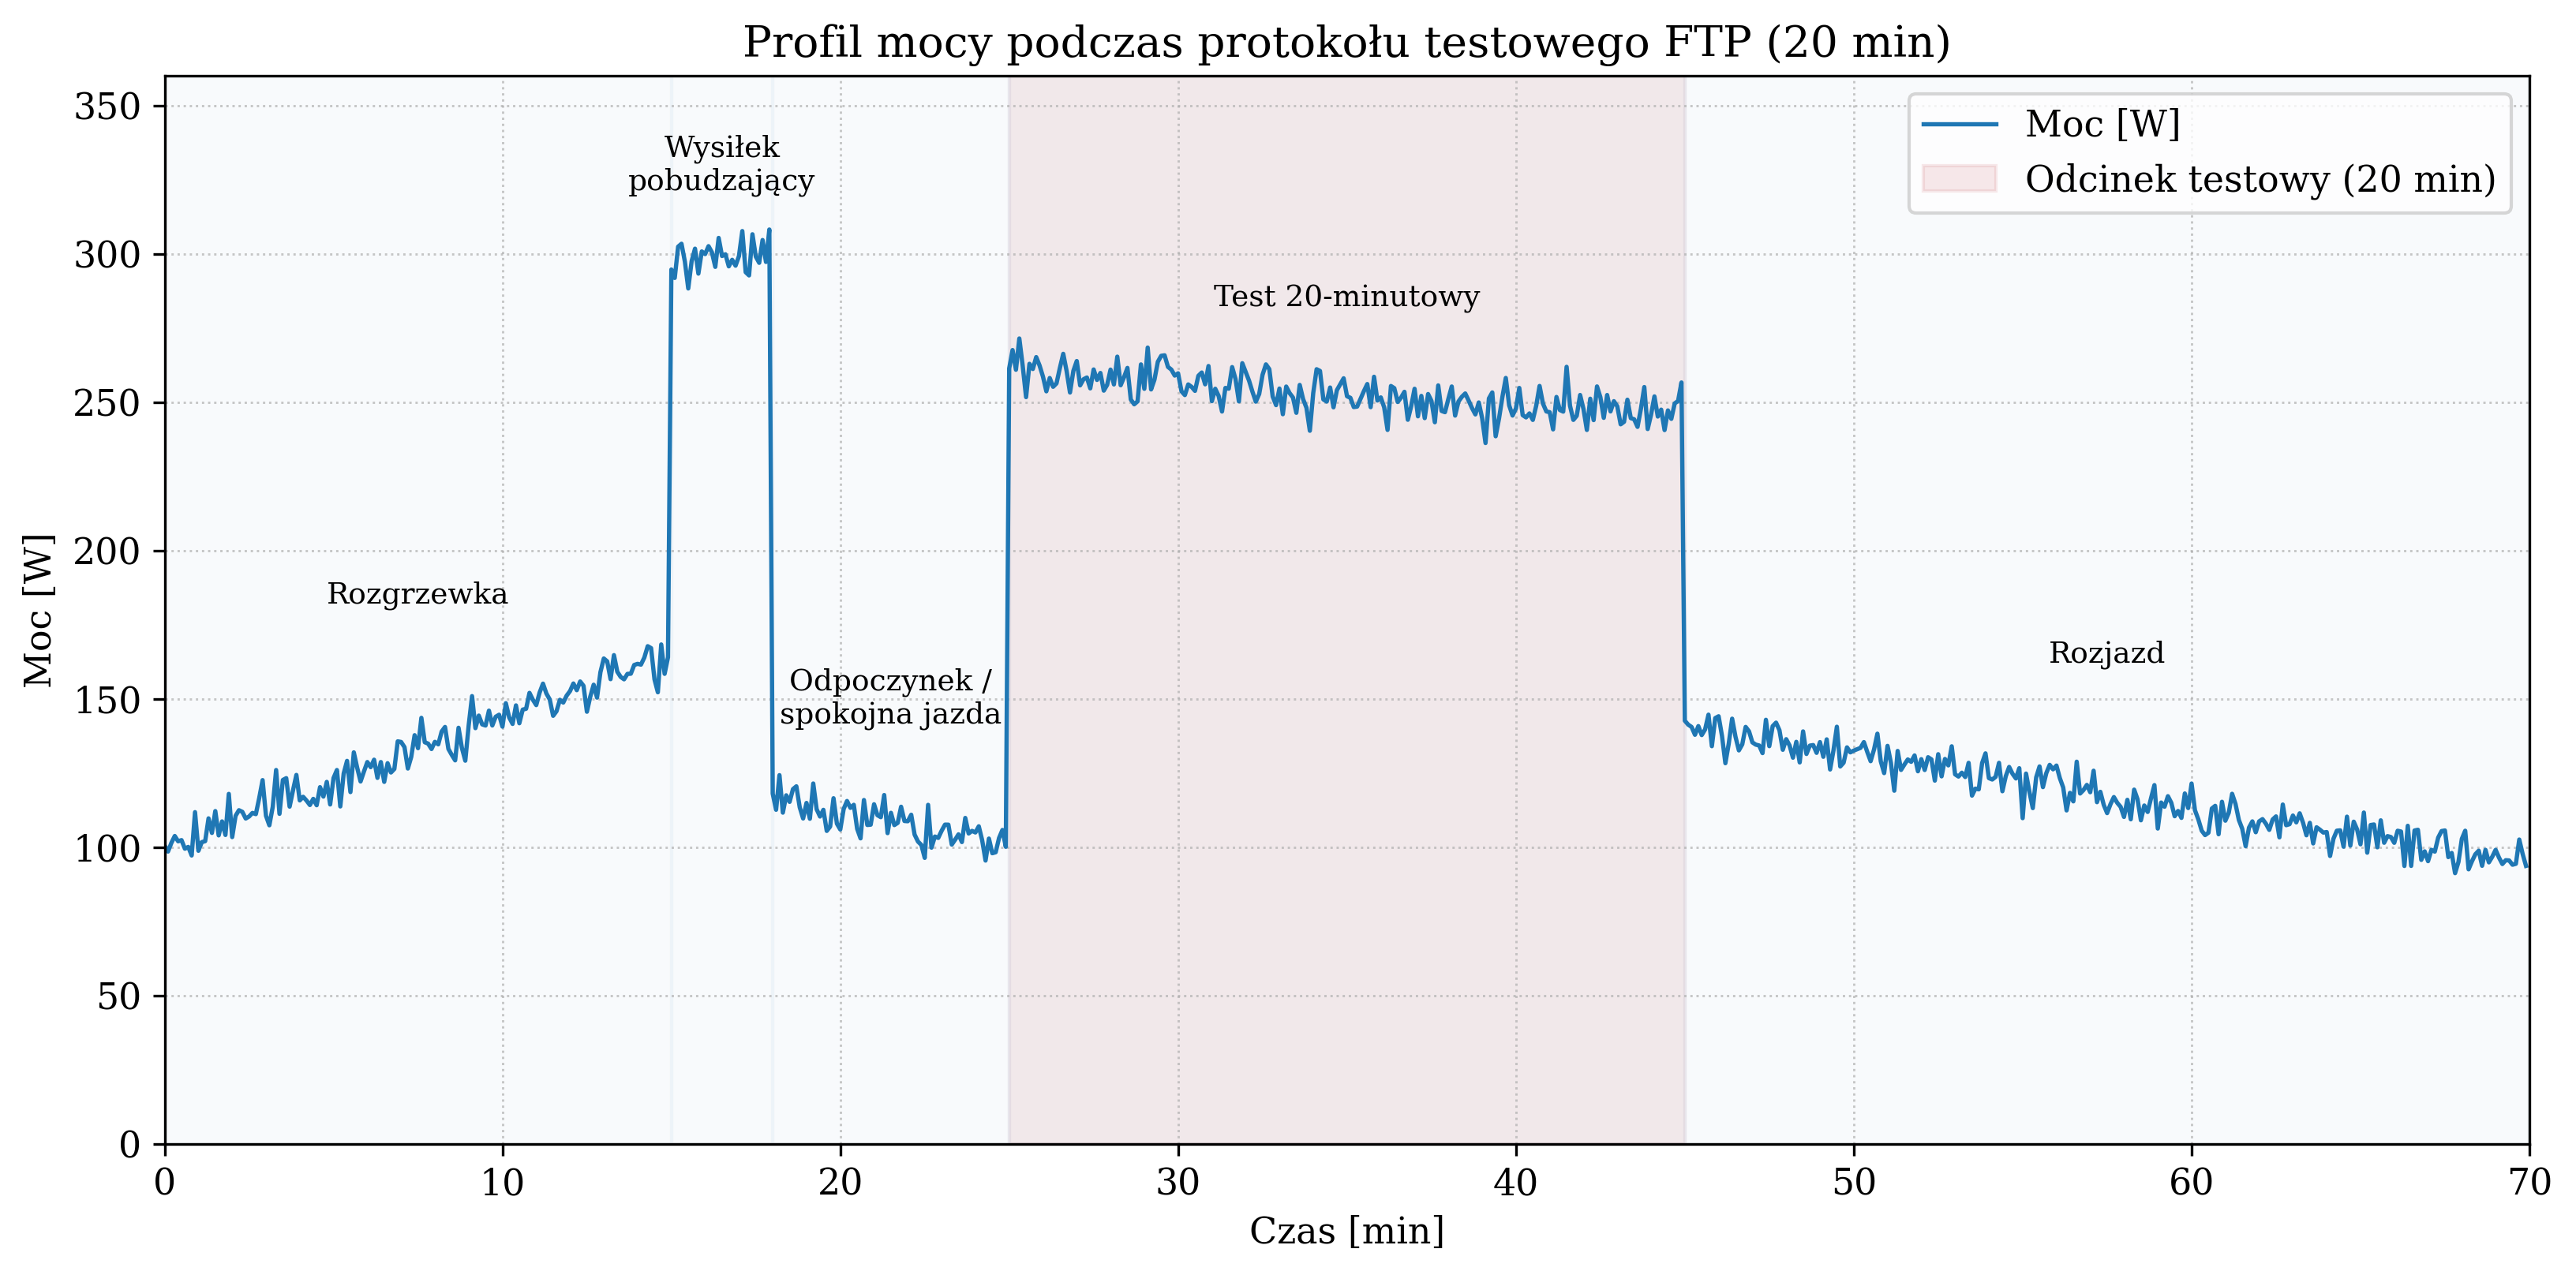
\includegraphics[width=0.95\linewidth]{figures/theory/ftp_20min_protocol.png}
  \caption[Schemat przebiegu testu 20-minutowego FTP]{Schemat przebiegu testu $20$-minutowego $\mathrm{FTP}$: rozgrzewka, wysiłek pobudzający, spokojna jazda, $20$-minutowy wysiłek testowy oraz rozjazd. Wynik z otrzymaną średnią należy przemnożyć przez $0{,}95$.\par Źródło: Opracowanie własne na podstawie \parencite{allen2019power}.}
  \label{fig:test_20min_schema}
\end{figure}

Zjawisko dryfu tętna ma znaczenie również przy interpretacji testów $20$-minutowych. Nawet przy względnie stabilnej mocy w części zasadniczej testu tętno może stopniowo wzrastać, co oznacza, że odpowiedź fizjologiczna organizmu nie jest stała w czasie. Z tego powodu cechy opisujące relację mocy i tętna powinny uwzględniać nie tylko wartości średnie, lecz także zmiany tej relacji w trakcie wysiłku.

Wynik próby zależy również od strategii tempa. Zbyt intensywny początek może doprowadzić do spadku mocy w końcowej części testu, natomiast nadmiernie zachowawcza jazda utrudnia wykorzystanie pełnego potencjału zawodnika. Porównywalność kolejnych pomiarów wymaga zbliżonych warunków, podobnego poziomu zmęczenia i właściwego przygotowania. Dla osoby trenującej rekreacyjnie spełnienie tych warunków przy regularnym powtarzaniu próby bywa trudne. Jest to jedna z przyczyn, dla których pasywna estymacja oparta na historii aktywności może stanowić wartościowe uzupełnienie formalnych testów.

\FloatBarrier
\subsection{Test 60-minutowy -- przebieg i ilustracja}

Choć w praktyce trenerskiej najczęściej stosuje się skrócone protokoły (np.\ test $20$-minutowy), pełny, $60$-minutowy test czasowy uznawany jest za najbardziej bezpośrednią i klasyczną metodę wyznaczania $\mathrm{FTP}$.
W ujęciu historycznym $\mathrm{FTP}$ definiowano jako moc, którą zawodnik jest w stanie utrzymać przez pełną godzinę jazdy ciągłej.
Wymaga to jednak bardzo wysokiej dyspozycji, odpowiedniego przygotowania mentalnego oraz sprzyjających warunków, dlatego test stosuje się głównie w środowisku laboratoryjnym lub u doświadczonych kolarzy \parencite{allen2019power,sitko2023_ac20to60_update}.

Klasyczna procedura wyznaczania FTP, oparta na pełnym wysiłku godzinnym, jest metodologicznie zbliżona do prób czasowych na dystansie godzinnym \parencite{allen2019power}. Strukturę tego testu można scharakteryzować następująco:
\begin{itemize}
  \item \textbf{Rozgrzewka i aktywacja} -- trwająca 15--20 minut jazda przygotowawcza o niskiej i średniej intensywności.
  \item \textbf{Etap przejściowy} -- 5--10 minut jazdy o minimalnej intensywności, służącej stabilizacji tętna przed główną próbą.
  \item \textbf{Próba zasadnicza} -- 60-minutowa ciągła jazda o maksymalnej możliwej do utrzymania mocy, gdzie średnia wartość mocy jest bezpośrednio przyjmowana jako FTP.
\end{itemize}

Przebieg pełnego testu $60$-minutowego przedstawiono na rysunku~\ref{fig:test_60min_schema}.
W przypadku pełnego testu 60-minutowego najważniejszym elementem jest godzinna część zasadnicza, w której zawodnik próbuje utrzymać możliwie stałą moc. Ze względu na długość i obciążenie test ten jest trudniejszy do częstego wykonywania niż protokół 20-minutowy.

\begin{figure}[htbp]
  \centering
  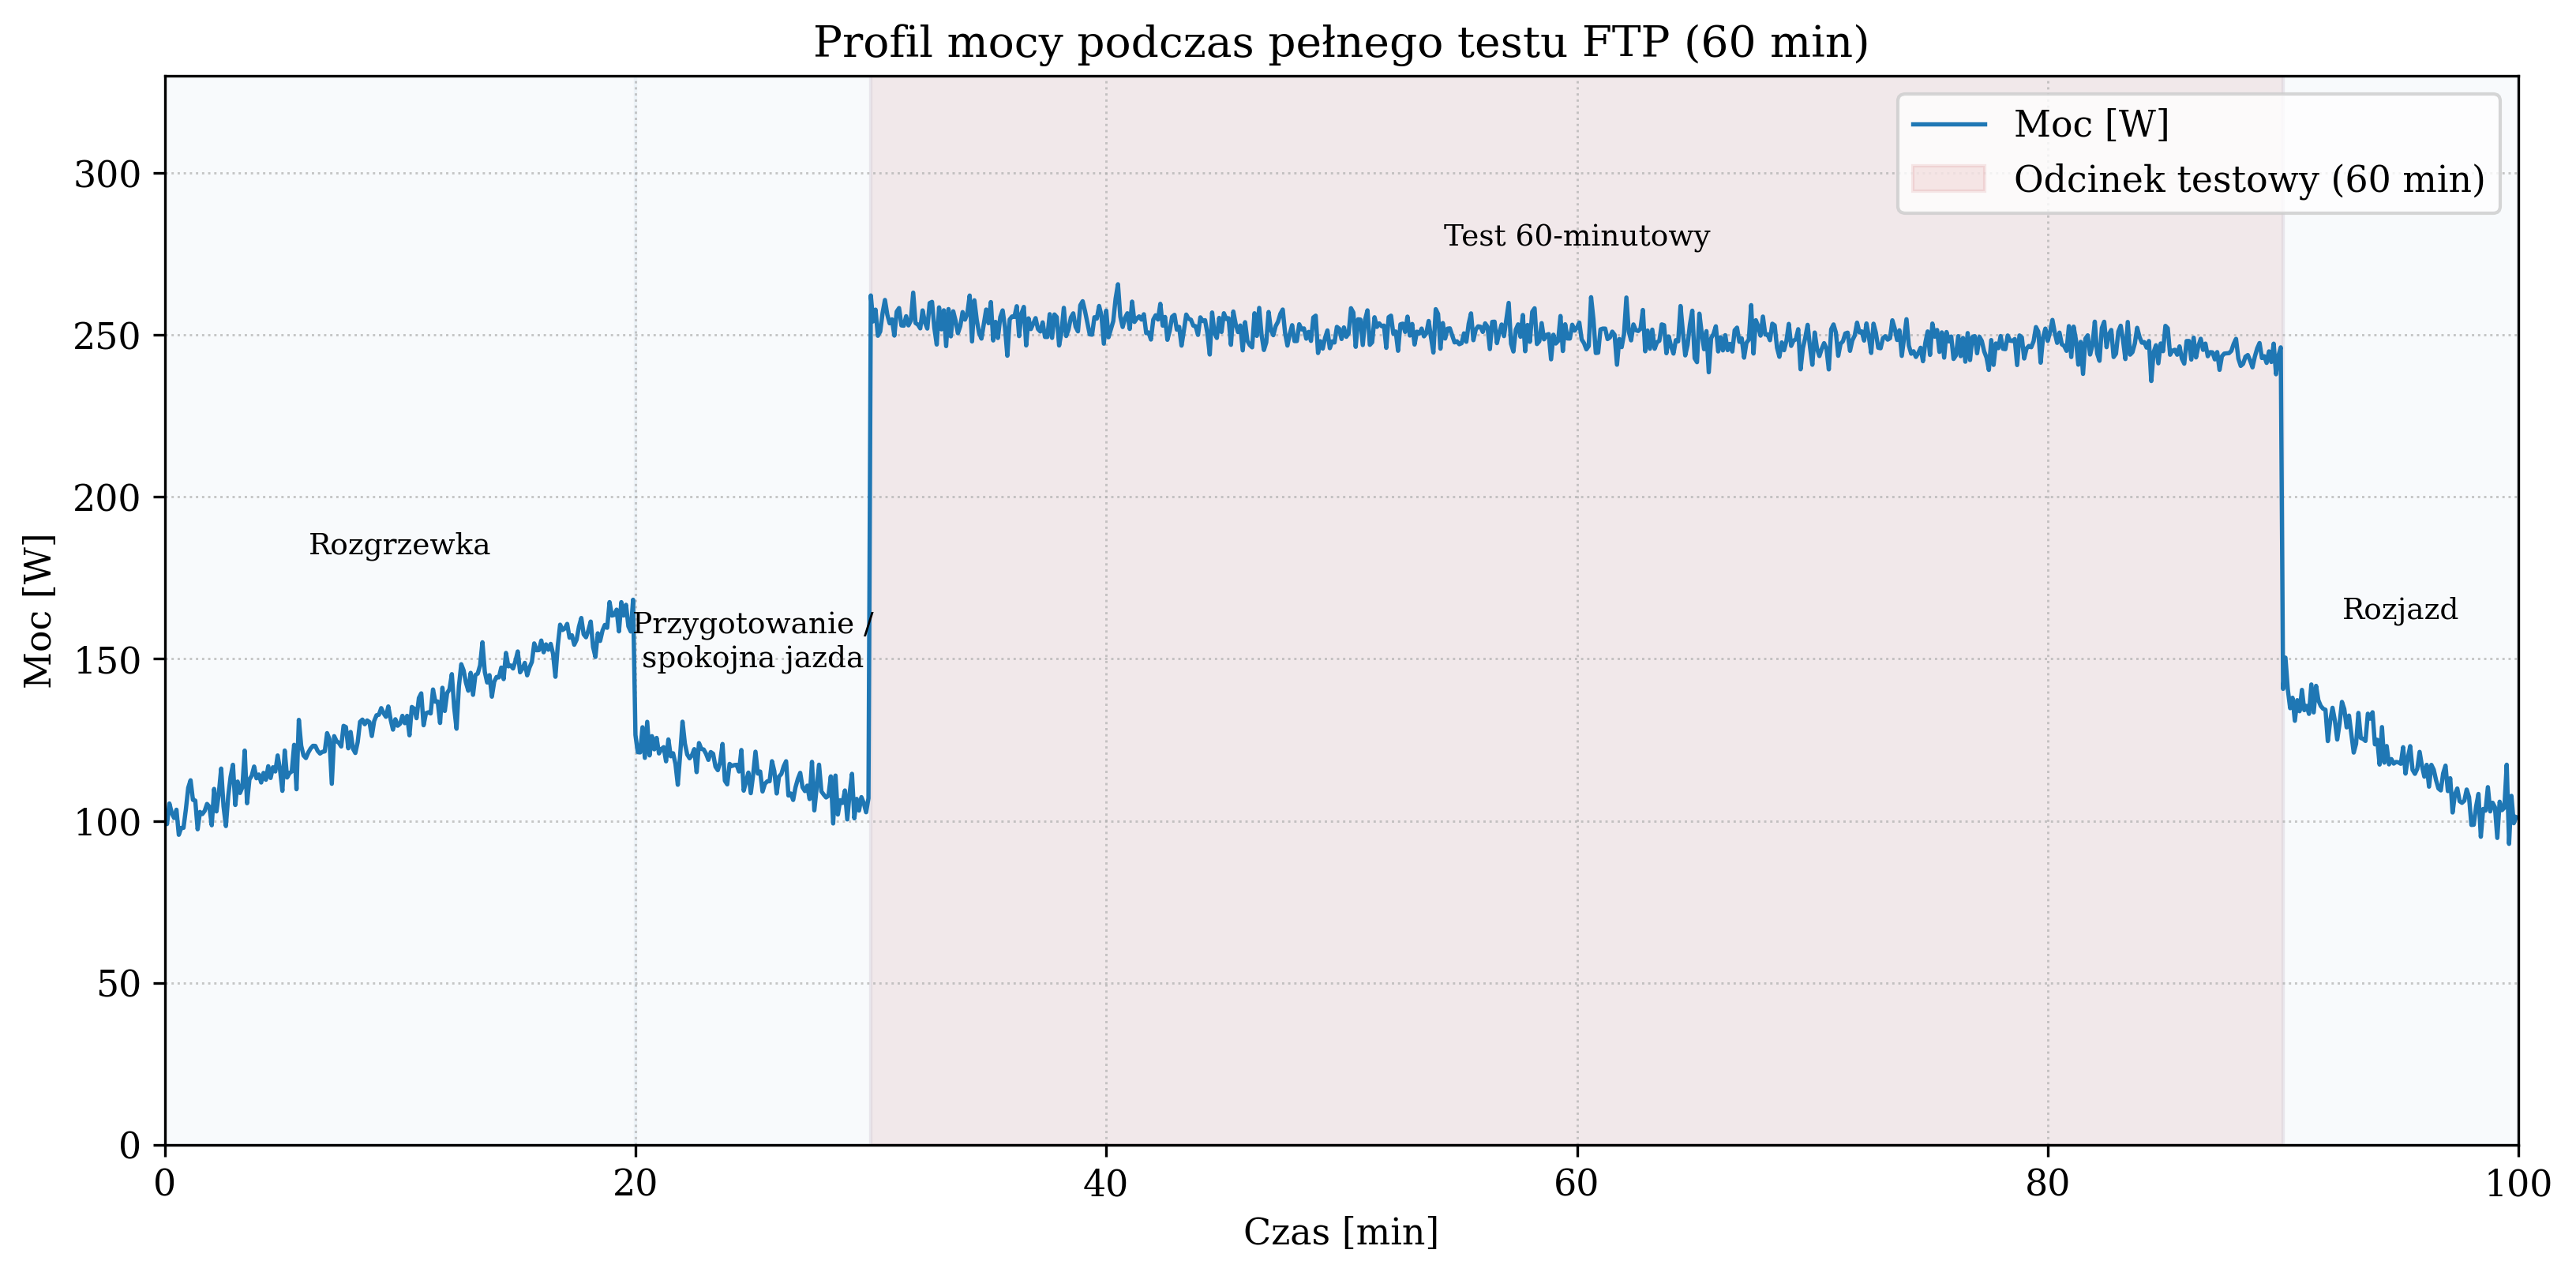
\includegraphics[width=0.95\linewidth]{figures/theory/ftp_60min_protocol.png}
  \caption[Schemat przebiegu pełnego testu 60-minutowego FTP]{Schemat przebiegu pełnego testu $60$-minutowego $\mathrm{FTP}$: rozgrzewka, przygotowanie połączone ze spokojną jazdą, główny godzinny odcinek o możliwie stałej mocy oraz rozjazd. Średnia moc z $60$-minutowego segmentu stanowi bezpośredni wyznacznik $\mathrm{FTP}$.\par Źródło: Opracowanie własne na podstawie \parencite{allen2019power}.}
  \label{fig:test_60min_schema}
\end{figure}

\FloatBarrier
\subsection{Krzywa mocy i zależność FTP od czasu trwania wysiłku}

Schematyczną zależność maksymalnej możliwej do utrzymania mocy od czasu trwania wysiłku przedstawiono na rysunku \ref{fig:power_duration_curve}.
Dla bardzo krótkich czasów wartości mocy są wysokie i szybko maleją, natomiast przy dłuższych wysiłkach krzywa stopniowo zbliża się do poziomu odpowiadającego mocy krytycznej ($\mathrm{CP}$), która jest blisko spokrewniona z funkcjonalnym progiem mocy ($\mathrm{FTP}$) \parencite{pinot2011recordPowerProfile,borszcz2018ftp,allen2019power,karsten2021cpftp}.
Krzywa mocy pokazuje, że maksymalna możliwa do utrzymania moc maleje wraz z wydłużaniem czasu wysiłku, a przy długich czasach zbliża się do poziomu odpowiadającego mocy progowej.

\begin{figure}[htbp]
  \centering
  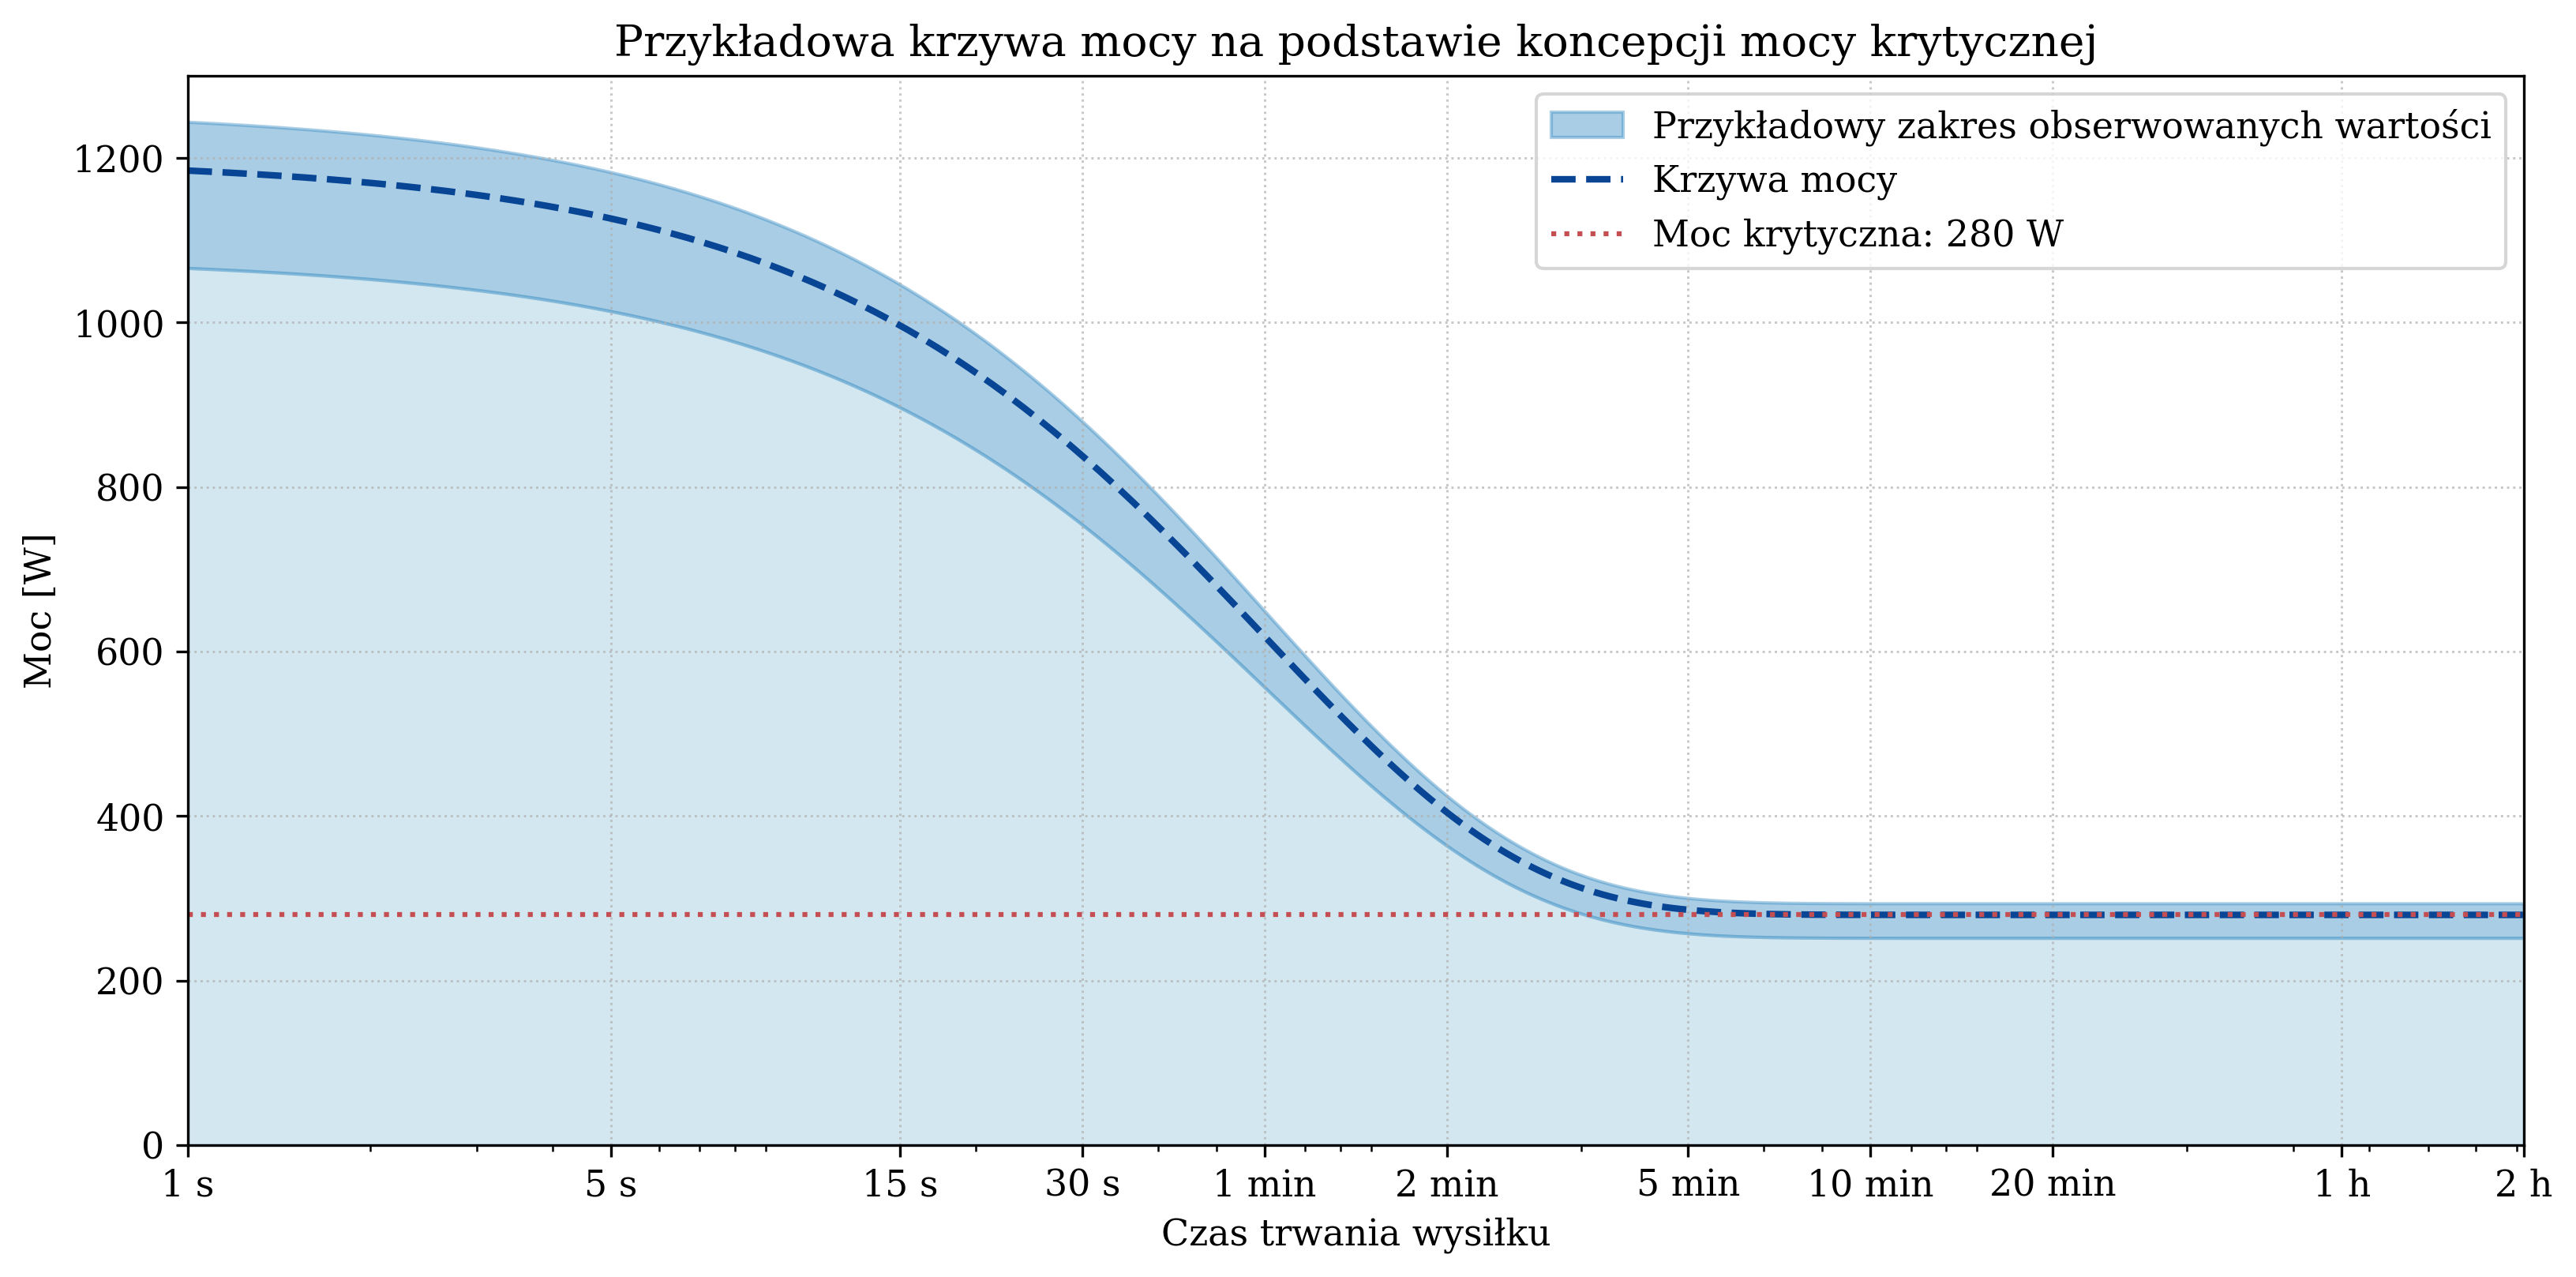
\includegraphics[width=0.95\linewidth]{figures/theory/power_duration_curve.png}
  \caption[Przykładowa krzywa mocy na podstawie koncepcji mocy krytycznej]{Przykładowa krzywa mocy przedstawiająca spadek maksymalnej możliwej do utrzymania mocy wraz z wydłużaniem czasu wysiłku.\par Źródło: Opracowanie własne na podstawie koncepcji mocy krytycznej.}
  \label{fig:power_duration_curve}
\end{figure}

\FloatBarrier
W praktyce platformy treningowe i oprogramowanie analityczne wykorzystują takie krzywe do estymacji parametrów wydolnościowych, w tym $\mathrm{FTP}$, na podstawie danych z wielu treningów bez konieczności wykonywania osobnego testu \parencite{borszcz2018ftp,allen2019power,karsten2021cpftp,denham2020predictftp}.

\section{Charakterystyka danych treningowych}

Modele uczenia maszynowego wykorzystywane do estymacji $\mathrm{FTP}$ opierają się na danych rejestrowanych podczas jazdy na rowerze.
Podstawowym źródłem informacji jest miernik mocy instalowany w korbie, piaście, pedale lub suporcie, który z wysoką częstotliwością (najczęściej $1\ \mathrm{Hz}$) rejestruje chwilową moc generowaną przez kolarza.
Równolegle rejestrowane jest tętno za pomocą opaski na klatkę piersiową lub optycznego czujnika na nadgarstku.
W zależności od konfiguracji sprzętu oraz platformy treningowej możliwe jest także zapisywanie dodatkowych parametrów, takich jak kadencja, prędkość, położenie GPS, nachylenie trasy czy wysokość nad poziomem morza \parencite{allen2019power,phasescycling2023_ftp_variability,kaggle_redlineracer_road_cycling_performance_testing,osf_goldencheetah_opendata}.

W kontekście uczenia maszynowego dane te mają postać szeregów czasowych: dla każdej sekundy otrzymujemy wektor obserwacji zawierający m.in.\ moc [$\mathrm{W}$], tętno [$\mathrm{bpm}$] oraz znacznik czasu.
Dodatkowo dostępne są metadane opisujące daną sesję: typ treningu (jazda spokojna, interwały, wyścig), użyty sprzęt, warunki pogodowe, a także informacja o zawodniku (masa ciała, kategoria wiekowa, poziom sportowy).
Otwarte zbiory danych wykorzystywane w literaturze oraz w niniejszej pracy obejmują zarówno pomiary wykonywane w warunkach laboratoryjnych, jak i dane z rzeczywistych treningów terenowych zapisane w formatach $\mathrm{GPX}$, $\mathrm{FIT}$ czy $\mathrm{CSV}$ \parencite{kaggle_redlineracer_road_cycling_performance_testing,osf_goldencheetah_opendata,stockwell2023mlftp}.

Kluczową relacją wykorzystywaną przez model jest zależność pomiędzy mocą a tętnem.
Moc odzwierciedla rzeczywistą pracę mechaniczną wykonywaną przez kolarza, natomiast tętno jest miarą reakcji układu krążenia na obciążenie wysiłkiem.
Zależność ta ma charakter nieliniowy i jest modulowana wieloma czynnikami, takimi jak temperatura, poziom odwodnienia, stan zmęczenia czy stosowane leki.
Dodatkowo w trakcie dłuższych wysiłków obserwuje się zjawisko dryfu tętna: stopniowego wzrostu częstości skurczów serca pomimo utrzymywania z grubsza stałej mocy \parencite{borszcz2018ftp,karsten2021cpftp}.
Zjawiska te sprawiają, że proste modele liniowe mogą okazać się niewystarczające, natomiast stanowią naturalne pole zastosowania metod uczenia maszynowego zdolnych do modelowania złożonych, nieliniowych zależności \parencite{stockwell2023mlftp,denham2020predictftp}.

Istotnym wyzwaniem jest jakość danych treningowych.
W realnych warunkach jazdy rejestrowane szeregi zawierają liczne fragmenty, które nie są bezpośrednio związane z wydolnością tlenową: zjazdy przy niskiej mocy, postoje na skrzyżowaniach, zakłócenia wynikające z utraty sygnału GPS lub błędów odczytu czujników.
Dodatkowo w otwartych zbiorach danych spotyka się brakujące wartości, niespójne nazewnictwo treningów oraz różne częstotliwości próbkowania.
Zanim dane zostaną wykorzystane w modelu, konieczne jest przeprowadzenie operacji wstępnego przetwarzania (filtrowanie, ujednolicanie częstotliwości próbkowania, uzupełnianie lub usuwanie braków oraz segmentacja jazd).

Poszczególne sygnały niosą odmienny rodzaj informacji i są obciążone innymi źródłami błędu. Moc reaguje szybko na zmianę nacisku na pedały, lecz zerowe wartości mogą oznaczać zarówno odpoczynek na zjeździe, jak i fragment jazdy bez pedałowania. Tętno opisuje odpowiedź organizmu, ale reaguje z opóźnieniem, a jego brak może wynikać z niezałożenia pasa lub przerwania transmisji. Kadencja pomaga odróżnić aktywne pedałowanie od toczenia roweru, lecz również zależy od działania czujnika. Prędkość i wysokość ułatwiają interpretację profilu trasy, ale podlegają wpływowi warunków zewnętrznych oraz jakości sygnału GPS. Znacznik czasu jest potrzebny do obliczania długości okien i agregacji, a jednocześnie ujawnia nieregularności próbkowania.

Dane terenowe są zatem bardziej zróżnicowane niż zapis próby laboratoryjnej prowadzonej na ergometrze. W laboratorium można kontrolować obciążenie, czas trwania stopni wysiłku, temperaturę oraz moment poboru próbek. W rzeczywistej jeździe występują zmiany nachylenia, ruch drogowy, wiatr i decyzje taktyczne zawodnika. Ta zmienność nie jest wyłącznie wadą: reprezentuje warunki, w których narzędzie miałoby działać. Wymaga jednak filtracji i inżynierii cech, aby model nie interpretował artefaktów pomiarowych jako informacji o wydolności.

\section{Klasyczne podejścia a uczenie maszynowe w szacowaniu FTP}

Tradycyjnie do wyznaczania $\mathrm{FTP}$ stosuje się metody oparte na prostych zależnościach matematycznych i z góry ustalonych protokołach testowych.
Przykładem jest $20$-minutowy test czasowy, w którym $\mathrm{FTP}$ definiuje się jako stały procent średniej mocy z próby \parencite{allen2019power,sitko2023_ac20to60_update,phasescycling2023_ftp_variability}.
Inne podejścia bazują na modelu mocy--czasu ($\mathrm{CP}$), gdzie na podstawie kilku testów o różnym czasie trwania estymuje się parametry krzywej opisującej zależność pomiędzy czasem wysiłku a możliwą do utrzymania mocą \parencite{denham2020predictftp}.
W diagnostyce sportowej wykorzystuje się również pułap tlenowy ($\text{VO}_{2\max}$), progi wentylacyjne ($\text{VT}_1$, $\text{VT}_2$) oraz progi mleczanowe ($\text{LT}_1$, $\text{LT}_2$). Wskaźniki te mają istotną wartość naukową i pozwalają precyzyjnie opisać reakcję organizmu na narastające obciążenie. Ich regularne wyznaczanie wymaga jednak laboratorium, specjalistycznej aparatury i obsługi, a w przypadku progów mleczanowych także pobierania próbek krwi. Testy są obciążające dla zawodnika, kosztowne i trudne do częstego powtarzania, szczególnie w sporcie amatorskim \parencite{borszcz2018ftp,karsten2021cpftp}.

Ocena laboratoryjna może obejmować analizator gazów oddechowych, ergometr umożliwiający kontrolę obciążenia, pomiar tętna oraz procedurę pobierania próbek krwi. Przeprowadzenie badania wymaga odpowiedniego przygotowania zawodnika i personelu, a wynik odnosi się do konkretnego dnia oraz przyjętego protokołu. Powtarzanie pełnej diagnostyki w krótkich odstępach czasu jest zwykle nieproporcjonalne do potrzeb amatora. Nawet w sporcie wyczynowym badania laboratoryjne planuje się w wybranych momentach cyklu treningowego, a bieżące monitorowanie opiera również na danych z treningów.

Zaletą klasycznych metod jest prostota interpretacji oraz możliwość odniesienia wyniku do mechanizmów fizjologicznych.
Jednocześnie podejścia te zakładają wykonanie jednego lub kilku wysiłków w kontrolowanych warunkach, a uzyskana wartość ma charakter punktowy: opisuje stan zawodnika w chwili testu.
Zmiany wydolności pomiędzy testami pozostają niewidoczne, co ogranicza możliwość ciągłego monitorowania formy \parencite{denham2020predictftp,phasescycling2023_ftp_variability}.
Ograniczenia te uzasadniają wykorzystanie danych telemetrycznych rejestrowanych w codziennych treningach oraz modeli uczenia maszynowego, które mogą agregować informacje z wielu sesji.

Rozwój uczenia maszynowego oraz dostęp do dużych zbiorów danych treningowych otwierają alternatywną ścieżkę: zamiast opierać się wyłącznie na dedykowanych testach, można wykorzystać informacje zawarte w codziennych jazdach.
W literaturze pojawiają się projekty open-source, w których na podstawie historii treningów buduje się modele regresyjne przewidujące wartość $\mathrm{FTP}$ wyznaczoną testem referencyjnym \parencite{stockwell2023mlftp,denham2020predictftp}.
Rozwiązania te stanowią naturalny punkt odniesienia dla niniejszej pracy i pokazują, że podejście oparte na danych ma potencjał praktycznego zastosowania.

Typowo stosowane modele można podzielić na dwie główne grupy:
\begin{itemize}
  \item \textbf{Modele oparte na cechach zagregowanych.} Z surowych szeregów czasowych wyznacza się zestaw cech opisujących jazdę lub jej fragment (np.\ średnia moc i tętno, maksymalna moc z $5$- czy $20$-minutowego okresu, czas w strefach, miary zmienności). Na tak przygotowanych danych uczone są algorytmy regresji, takie jak regresja liniowa, Random Forest czy modele Gradient Boosting (np.\ XGBoost). Zaletą jest interpretowalność i relatywnie niewielkie wymagania obliczeniowe \parencite{stockwell2023mlftp}.
  \item \textbf{Modele sekwencyjne.} Podejście polega na bezpośrednim modelowaniu szeregów czasowych (bez redukcji do kilku wskaźników). Wykorzystuje się architektury neuronowe takie jak $\mathrm{LSTM}$, $\mathrm{GRU}$ czy modele typu \textit{Transformer} przystosowane do danych czasowych. Umożliwia to uchwycenie złożonych wzorców dynamiki wysiłku, jednak wymaga większej ilości danych, starannego doboru hiperparametrów i jest trudniejsze do interpretacji \parencite{stockwell2023mlftp}.
\end{itemize}

Oba podejścia nie wykluczają się wzajemnie.
W praktyce często tworzy się hybrydowe pipeline'y, w których część informacji pochodzi z cech zagregowanych, a część z modeli sekwencyjnych.
W niniejszej pracy przyjęto podejście regresyjne, w którym $\mathrm{FTP}$ traktowane jest jako zmienna ciągła, a celem jest minimalizacja błędu predykcji względem wartości referencyjnych wyznaczonych testami.

Wybór algorytmu do estymacji parametrów fizjologicznych jest kluczowy dla skuteczności modelu.
W literaturze przedmiotu najczęściej wymienia się następujące podejścia \parencite{stockwell2023mlftp}:

\paragraph{Modele liniowe i regularyzacja.}

Podstawowym narzędziem w zadaniach predykcji wartości ciągłej (jaką jest $\mathrm{FTP}$) jest regresja liniowa.
Zakłada ona liniową zależność między cechami wejściowymi (np.\ średnim tętnem, mocą z określonych przedziałów czasowych) a zmienną celu.
Choć fizjologia wysiłku ma charakter nieliniowy, modele liniowe stanowią dobry punkt odniesienia.
Aby zapobiec przeuczeniu przy dużej liczbie skorelowanych cech, stosuje się regularyzację:
\begin{itemize}
  \item \textbf{Lasso} ($\ell_1$) - umożliwia selekcję cech poprzez zerowanie współczynników przy mniej istotnych zmiennych,
  \item \textbf{Ridge} ($\ell_2$) - zmniejsza wariancję modelu, co jest korzystne przy współliniowości danych treningowych.
\end{itemize}

\paragraph{Metody zespołowe.}

Jednymi z najskuteczniejszych algorytmów w pracy z danymi tabelarycznymi są metody oparte na drzewach decyzyjnych.
Pojedyncze drzewo ma tendencję do nadmiernego dopasowania, dlatego stosuje się:
\begin{itemize}
  \item \textbf{Random Forest}, czyli metoda lasu losowego - wykorzystuje agregację bootstrapową, buduje wiele drzew decyzyjnych na losowych podzbiorach danych i cech, a następnie uśrednia predykcje. Dzięki temu jest odporniejsza na przeuczenie niż pojedyncze drzewo i dobrze sprawdza się w danych tabelarycznych zawierających zależności nieliniowe.
  \item \textbf{Gradient Boosting} - buduje drzewa sekwencyjnie, a kolejne drzewa korygują błędy predykcji popełnione przez wcześniejsze elementy modelu. XGBoost jest wydajną implementacją tego podejścia, rozwiniętą z myślą o skutecznym uczeniu na danych tabelarycznych.
\end{itemize}

W części empirycznej pracy modele Random Forest i XGBoost wykorzystano do regresyjnej estymacji FTP, natomiast Ridge Regression pełni rolę liniowego punktu odniesienia.

\paragraph{Ryzyko wycieku danych.}

W zadaniach predykcyjnych należy oddzielić informację dostępną w rzeczywistym zastosowaniu od informacji, która powstała bezpośrednio podczas tworzenia etykiety. Wyciek danych (ang.\ \textit{data leakage}) występuje wtedy, gdy predyktor przekazuje modelowi część odpowiedzi lub pozwala ją odtworzyć w sposób niedostępny w docelowym scenariuszu. Skutkiem może być bardzo wysoka wartość $R^2$ i niski błąd, które nie świadczą o generalizacji modelu \parencite{kaufman2012leakage,bernett2024leakage}.

W przypadku heurystycznego FTP ryzyko jest szczególnie wyraźne. Jeżeli wartość referencyjną obliczono jako $0{,}95$ maksymalnej średniej mocy 20-minutowej, pozostawienie cechy \texttt{mmp\_20min} w zbiorze wejściowym umożliwia niemal bezpośrednie odtworzenie etykiety. Kontrola listy cech jest zatem równie ważna jak wybór algorytmu i metryk. Sama wysoka jakość dopasowania nie wystarcza do uznania eksperymentu za wiarygodny, jeżeli nie zbadano pochodzenia predyktorów oraz sposobu podziału danych.

\paragraph{Sieci neuronowe i głębokie uczenie.}

Gdy dane wejściowe traktujemy jako surowy szereg czasowy (sekwencja próbek moc/tętno co $1$ sekundę), intensywna inżynieria cech może prowadzić do utraty informacji o dynamice zmian.
W takich przypadkach zastosowanie znajdują:
\begin{itemize}
  \item rekurencyjne sieci neuronowe ($\mathrm{RNN}$) oraz $\mathrm{LSTM}$,
  \item konwolucyjne sieci neuronowe $1\mathrm{D}$ ($1\mathrm{D}$-$\mathrm{CNN}$),
  \item modele typu \textit{Transformer} dla szeregów czasowych.
\end{itemize}

\section{Zarys procesu przetwarzania danych i budowy modelu}

Zastosowanie uczenia maszynowego do estymacji $\mathrm{FTP}$ wymaga zdefiniowania spójnego procesu przetwarzania danych obejmującego następujące etapy.

\paragraph{Pozyskanie i integracja danych.}
W pracy wykorzystano otwarte zbiory danych zawierające zarówno wyniki testów wydolnościowych, jak i towarzyszące im szeregi czasowe mocy oraz tętna \parencite{kaggle_redlineracer_road_cycling_performance_testing,osf_goldencheetah_opendata,stockwell2023mlftp}.
Uzupełnieniem są pliki $\mathrm{GPX}/\mathrm{FIT}$ z regularnych jazd terenowych, przetworzone w ramach potoku ETL opisanego w rozdziale drugim.

\paragraph{Przygotowanie danych.}
Przygotowanie danych (ang.\ \textit{preprocessing}) obejmuje m.in.\ filtrację artefaktów pomiarowych, ujednolicenie częstotliwości próbkowania oraz obsługę brakujących wartości.
Jakość tego etapu ma bezpośredni wpływ na stabilność cech i modeli.

\paragraph{Definicja etykiet.}
Naturalnym wyborem jest $\mathrm{FTP}$ wyznaczone na podstawie standaryzowanego testu referencyjnego (np.\ testu $20$-minutowego skorygowanego współczynnikiem) lub wyniku laboratoryjnego odpowiadającego mocy progowej \parencite{borszcz2018ftp,karsten2021cpftp,denham2020predictftp}.
Następnie dla treningów wykonywanych w określonym oknie czasowym względem testu (np.\ $\pm 2$ tygodnie) przyjmuje się tę samą wartość $\mathrm{FTP}$, co pozwala przypisać etykietę do wielu sesji bez wykonywania dodatkowych testów \parencite{stockwell2023mlftp,denham2020predictftp}.
Jest to świadome założenie modelowe: w krótkim horyzoncie czasu $\mathrm{FTP}$ zmienia się relatywnie wolno.

\paragraph{Inżynieria cech.}
Inżynieria cech (ang.\ \textit{feature engineering}) polega na wyznaczeniu z surowych danych cech opisujących wysiłek i reakcję organizmu: średnich i maksymalnych mocy w oknach czasowych, rozkładu czasu w strefach, relacji mocy do tętna, miar zmienności tętna oraz wskaźników dryfu tętna.

\paragraph{Trening i ewaluacja.}
W zależności od projektu badania zbiór danych może zostać podzielony z uwzględnieniem grupowania obserwacji na poziomie zawodnika lub bloku czasowego.
W finalnym eksperymencie opisanym w niniejszej pracy zastosowano pojedynczy podział treningowy i testowy z użyciem mechanizmu \texttt{GroupShuffleSplit} grupującego obserwacje po zawodniku. Takie rozwiązanie ogranicza ryzyko wycieku informacji pomiędzy sesjami tej samej osoby \parencite{tougui2021crossValidation,rosenblatt2024leakage}.
Jako miary jakości predykcji stosuje się typowo $\mathrm{MAE}$, $\mathrm{RMSE}$ oraz miary korelacji i determinacji, w tym $R^2$ \parencite{chai2014rmseMae,james2021isl,hastie2009esl}.

\paragraph{Metryki ewaluacji modelu.}
Aby obiektywnie ocenić jakość estymacji $\mathrm{FTP}$ przez model, konieczne jest zdefiniowanie miar błędu.
W problemach regresji standardowo stosuje się m.in.\ następujące metryki \parencite{james2021isl,hastie2009esl}.

Metryki te obejmują:

\begin{equation}
\label{eq:rmse}
\mathrm{RMSE} = \sqrt{\frac{1}{n}\sum_{i=1}^{n}\left(y_i - \hat{y}_i\right)^2},
\end{equation}
gdzie $y_i$ oznacza rzeczywistą wartość $\mathrm{FTP}$ (wyznaczoną na podstawie testu referencyjnego), a $\hat{y}_i$ odpowiadającą jej wartość przewidywaną przez model.
$\mathrm{RMSE}$ jest wrażliwy na duże błędy (obserwacje odstające), co jest pożądane w zastosowaniach sportowych, ponieważ duże pomyłki mogłyby prowadzić do niewłaściwego doboru obciążeń treningowych.

\paragraph{Średni błąd bezwzględny (MAE).}
\begin{equation}
\label{eq:mae}
\mathrm{MAE} = \frac{1}{n}\sum_{i=1}^{n}\left|y_i - \hat{y}_i\right|.
\end{equation}
$\mathrm{MAE}$ jest łatwiejsze w interpretacji dla trenera, ponieważ wprost mówi, o ile watów średnio myli się model (np.\ „średni błąd wynosi $5\ \mathrm{W}$”).

\paragraph{Współczynnik determinacji ($R^2$).}
\begin{equation}
\label{eq:r2}
R^2 = 1 - \frac{\sum_{i=1}^{n}\left(y_i - \hat{y}_i\right)^2}{\sum_{i=1}^{n}\left(y_i - \bar{y}\right)^2},
\end{equation}
gdzie $\bar{y}$ oznacza średnią wartość rzeczywistego $\mathrm{FTP}$ w próbie.
Wartość bliska $R^2 = 1$ oznacza bardzo dobre dopasowanie modelu do danych, natomiast wartości ujemne świadczą o tym, że model przewiduje gorzej niż proste przyjęcie średniej z próby.
W badaniach nad wydolnością wysokie wartości $R^2$ (np.\ powyżej $0{,}9$) pomiędzy wynikami testów skróconych a pełnymi bywają interpretowane jako przesłanka użyteczności danej metody estymacji \parencite{karsten2021cpftp}.
